\documentclass[1p]{elsarticle_modified}
%\bibliographystyle{elsarticle-num}

%\usepackage[colorlinks]{hyperref}
%\usepackage{abbrmath_seonhwa} %\Abb, \Ascr, \Acal ,\Abf, \Afrak
\usepackage{amsfonts}
\usepackage{amssymb}
\usepackage{amsmath}
\usepackage{amsthm}
\usepackage{scalefnt}
\usepackage{amsbsy}
\usepackage{kotex}
\usepackage{caption}
\usepackage{subfig}
\usepackage{color}
\usepackage{graphicx}
\usepackage{xcolor} %% white, black, red, green, blue, cyan, magenta, yellow
\usepackage{float}
\usepackage{setspace}
\usepackage{hyperref}

\usepackage{tikz}
\usetikzlibrary{arrows}

\usepackage{multirow}
\usepackage{array} % fixed length table
\usepackage{hhline}

%%%%%%%%%%%%%%%%%%%%%
\makeatletter
\renewcommand*\env@matrix[1][\arraystretch]{%
	\edef\arraystretch{#1}%
	\hskip -\arraycolsep
	\let\@ifnextchar\new@ifnextchar
	\array{*\c@MaxMatrixCols c}}
\makeatother %https://tex.stackexchange.com/questions/14071/how-can-i-increase-the-line-spacing-in-a-matrix
%%%%%%%%%%%%%%%

\usepackage[normalem]{ulem}

\newcommand{\msout}[1]{\ifmmode\text{\sout{\ensuremath{#1}}}\else\sout{#1}\fi}
%SOURCE: \msout is \stkout macro in https://tex.stackexchange.com/questions/20609/strikeout-in-math-mode

\newcommand{\cancel}[1]{
	\ifmmode
	{\color{red}\msout{#1}}
	\else
	{\color{red}\sout{#1}}
	\fi
}

\newcommand{\add}[1]{
	{\color{blue}\uwave{#1}}
}

\newcommand{\replace}[2]{
	\ifmmode
	{\color{red}\msout{#1}}{\color{blue}\uwave{#2}}
	\else
	{\color{red}\sout{#1}}{\color{blue}\uwave{#2}}
	\fi
}

\newcommand{\Sol}{\mathcal{S}} %segment
\newcommand{\D}{D} %diagram
\newcommand{\A}{\mathcal{A}} %arc


%%%%%%%%%%%%%%%%%%%%%%%%%%%%%5 test

\def\sl{\operatorname{\textup{SL}}(2,\Cbb)}
\def\psl{\operatorname{\textup{PSL}}(2,\Cbb)}
\def\quan{\mkern 1mu \triangleright \mkern 1mu}

\theoremstyle{definition}
\newtheorem{thm}{Theorem}[section]
\newtheorem{prop}[thm]{Proposition}
\newtheorem{lem}[thm]{Lemma}
\newtheorem{ques}[thm]{Question}
\newtheorem{cor}[thm]{Corollary}
\newtheorem{defn}[thm]{Definition}
\newtheorem{exam}[thm]{Example}
\newtheorem{rmk}[thm]{Remark}
\newtheorem{alg}[thm]{Algorithm}

\newcommand{\I}{\sqrt{-1}}
\begin{document}

%\begin{frontmatter}
%
%\title{Boundary parabolic representations of knots up to 8 crossings}
%
%%% Group authors per affiliation:
%\author{Yunhi Cho} 
%\address{Department of Mathematics, University of Seoul, Seoul, Korea}
%\ead{yhcho@uos.ac.kr}
%
%
%\author{Seonhwa Kim} %\fnref{s_kim}}
%\address{Center for Geometry and Physics, Institute for Basic Science, Pohang, 37673, Korea}
%\ead{ryeona17@ibs.re.kr}
%
%\author{Hyuk Kim}
%\address{Department of Mathematical Sciences, Seoul National University, Seoul 08826, Korea}
%\ead{hyukkim@snu.ac.kr}
%
%\author{Seokbeom Yoon}
%\address{Department of Mathematical Sciences, Seoul National University, Seoul, 08826,  Korea}
%\ead{sbyoon15@snu.ac.kr}
%
%\begin{abstract}
%We find all boundary parabolic representation of knots up to 8 crossings.
%
%\end{abstract}
%\begin{keyword}
%    \MSC[2010] 57M25 
%\end{keyword}
%
%\end{frontmatter}

%\linenumbers
%\tableofcontents
%
\newcommand\colored[1]{\textcolor{white}{\rule[-0.35ex]{0.8em}{1.4ex}}\kern-0.8em\color{red} #1}%
%\newcommand\colored[1]{\textcolor{white}{ #1}\kern-2.17ex	\textcolor{white}{ #1}\kern-1.81ex	\textcolor{white}{ #1}\kern-2.15ex\color{red}#1	}

{\Large $\underline{11a_{46}~(K11a_{46})}$}

\setlength{\tabcolsep}{10pt}
\renewcommand{\arraystretch}{1.6}
\vspace{1cm}\begin{tabular}{m{100pt}>{\centering\arraybackslash}m{274pt}}
\multirow{5}{120pt}{
	\centering
	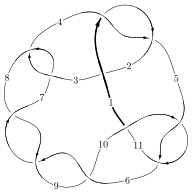
\includegraphics[width=112pt]{../../../GIT/diagram.site/Diagrams/png/295_11a_46.png}\\
\ \ \ A knot diagram\footnotemark}&
\allowdisplaybreaks
\textbf{Linearized knot diagam} \\
\cline{2-2}
 &
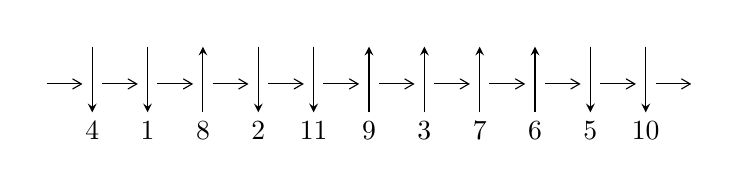
\begin{tikzpicture}[x=20pt, y=17pt]
	% nodes
	\node (C0) at (0, 0) {};
	\node (C1) at (1, 0) {};
	\node (C1U) at (1, +1) {};
	\node (C1D) at (1, -1) {4};

	\node (C2) at (2, 0) {};
	\node (C2U) at (2, +1) {};
	\node (C2D) at (2, -1) {1};

	\node (C3) at (3, 0) {};
	\node (C3U) at (3, +1) {};
	\node (C3D) at (3, -1) {8};

	\node (C4) at (4, 0) {};
	\node (C4U) at (4, +1) {};
	\node (C4D) at (4, -1) {2};

	\node (C5) at (5, 0) {};
	\node (C5U) at (5, +1) {};
	\node (C5D) at (5, -1) {11};

	\node (C6) at (6, 0) {};
	\node (C6U) at (6, +1) {};
	\node (C6D) at (6, -1) {9};

	\node (C7) at (7, 0) {};
	\node (C7U) at (7, +1) {};
	\node (C7D) at (7, -1) {3};

	\node (C8) at (8, 0) {};
	\node (C8U) at (8, +1) {};
	\node (C8D) at (8, -1) {7};

	\node (C9) at (9, 0) {};
	\node (C9U) at (9, +1) {};
	\node (C9D) at (9, -1) {6};

	\node (C10) at (10, 0) {};
	\node (C10U) at (10, +1) {};
	\node (C10D) at (10, -1) {5};

	\node (C11) at (11, 0) {};
	\node (C11U) at (11, +1) {};
	\node (C11D) at (11, -1) {10};
	\node (C12) at (12, 0) {};

	% arrows
	\draw[->,>={angle 60}]
	(C0) edge (C1) (C1) edge (C2) (C2) edge (C3) (C3) edge (C4) (C4) edge (C5) (C5) edge (C6) (C6) edge (C7) (C7) edge (C8) (C8) edge (C9) (C9) edge (C10) (C10) edge (C11) (C11) edge (C12) ;	\draw[->,>=stealth]
	(C1U) edge (C1D) (C2U) edge (C2D) (C3D) edge (C3U) (C4U) edge (C4D) (C5U) edge (C5D) (C6D) edge (C6U) (C7D) edge (C7U) (C8D) edge (C8U) (C9D) edge (C9U) (C10U) edge (C10D) (C11U) edge (C11D) ;
	\end{tikzpicture} \\
\hhline{~~} \\& 
\textbf{Solving Sequence} \\ \cline{2-2} 
 &
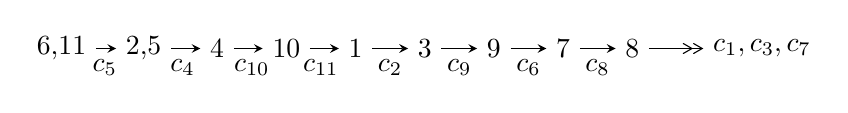
\begin{tikzpicture}[x=25pt, y=7pt]
	% node
	\node (A0) at (-1/8, 0) {6,11};
	\node (A1) at (17/16, 0) {2,5};
	\node (A2) at (17/8, 0) {4};
	\node (A3) at (25/8, 0) {10};
	\node (A4) at (33/8, 0) {1};
	\node (A5) at (41/8, 0) {3};
	\node (A6) at (49/8, 0) {9};
	\node (A7) at (57/8, 0) {7};
	\node (A8) at (65/8, 0) {8};
	\node (C1) at (1/2, -1) {$c_{5}$};
	\node (C2) at (13/8, -1) {$c_{4}$};
	\node (C3) at (21/8, -1) {$c_{10}$};
	\node (C4) at (29/8, -1) {$c_{11}$};
	\node (C5) at (37/8, -1) {$c_{2}$};
	\node (C6) at (45/8, -1) {$c_{9}$};
	\node (C7) at (53/8, -1) {$c_{6}$};
	\node (C8) at (61/8, -1) {$c_{8}$};
	\node (A9) at (10, 0) {$c_{1},c_{3},c_{7}$};

	% edge
	\draw[->,>=stealth]	
	(A0) edge (A1) (A1) edge (A2) (A2) edge (A3) (A3) edge (A4) (A4) edge (A5) (A5) edge (A6) (A6) edge (A7) (A7) edge (A8) ;
	\draw[->>,>={angle 60}]	
	(A8) edge (A9);
\end{tikzpicture} \\ 

\end{tabular} \\

\footnotetext{
The image of knot diagram is generated by the software ``\textbf{Draw programme}" developed by Andrew Bartholomew(\url{http://www.layer8.co.uk/maths/draw/index.htm\#Running-draw}), where we modified some parts for our purpose(\url{https://github.com/CATsTAILs/LinksPainter}).
}\phantom \\ \newline 
\centering \textbf{Ideals for irreducible components\footnotemark of $X_{\text{par}}$} 
 
\begin{align*}
I^u_{1}&=\langle 
- u^{15}- u^{14}+3 u^{13}+4 u^{12}-4 u^{11}-7 u^{10}- u^9+4 u^8+4 u^7+2 u^6-4 u^5-4 u^4- u^3+u^2+b,\\
\phantom{I^u_{1}}&\phantom{= \langle  }u^{15}+u^{14}-3 u^{13}-4 u^{12}+4 u^{11}+7 u^{10}+u^9-4 u^8-4 u^7-2 u^6+4 u^5+4 u^4+2 u^3- u^2+a,\\
\phantom{I^u_{1}}&\phantom{= \langle  }u^{16}+u^{15}-4 u^{14}-5 u^{13}+7 u^{12}+11 u^{11}-3 u^{10}-11 u^9-5 u^8+2 u^7+8 u^6+6 u^5-2 u^4-5 u^3- u^2+u+1\rangle \\
I^u_{2}&=\langle 
- u^{26}+8 u^{24}+\cdots+3 u^2+b,\;2 u^{27}+u^{26}+\cdots+a-3,\;u^{28}+u^{27}+\cdots-2 u-1\rangle \\
I^u_{3}&=\langle 
b-1,\;a+2,\;u-1\rangle \\
\\
\end{align*}
\raggedright * 3 irreducible components of $\dim_{\mathbb{C}}=0$, with total 45 representations.\\
\footnotetext{All coefficients of polynomials are rational numbers. But the coefficients are sometimes approximated in decimal forms when there is not enough margin.}
\newpage
\renewcommand{\arraystretch}{1}
\centering \section*{I. $I^u_{1}= \langle - u^{15}- u^{14}+\cdots+u^2+b,\;u^{15}+u^{14}+\cdots- u^2+a,\;u^{16}+u^{15}+\cdots+u+1 \rangle$}
\flushleft \textbf{(i) Arc colorings}\\
\begin{tabular}{m{7pt} m{180pt} m{7pt} m{180pt} }
\flushright $a_{6}=$&$\begin{pmatrix}1\\0\end{pmatrix}$ \\
\flushright $a_{11}=$&$\begin{pmatrix}0\\u\end{pmatrix}$ \\
\flushright $a_{2}=$&$\begin{pmatrix}- u^{15}- u^{14}+\cdots-2 u^3+u^2\\u^{15}+u^{14}+\cdots+u^3- u^2\end{pmatrix}$ \\
\flushright $a_{5}=$&$\begin{pmatrix}1\\- u^2\end{pmatrix}$ \\
\flushright $a_{4}=$&$\begin{pmatrix}u^{14}+u^{13}+\cdots+u^2- u\\- u^{14}- u^{13}+\cdots+u+1\end{pmatrix}$ \\
\flushright $a_{10}=$&$\begin{pmatrix}u\\- u^3+u\end{pmatrix}$ \\
\flushright $a_{1}=$&$\begin{pmatrix}- u^3\\u^5- u^3+u\end{pmatrix}$ \\
\flushright $a_{3}=$&$\begin{pmatrix}- u^{15}- u^{14}+\cdots-2 u^3+u^2\\u^{15}+u^{14}+\cdots+4 u^4- u^2\end{pmatrix}$ \\
\flushright $a_{9}=$&$\begin{pmatrix}u^3\\- u^3+u\end{pmatrix}$ \\
\flushright $a_{7}=$&$\begin{pmatrix}u^6- u^4+1\\- u^6+2 u^4- u^2\end{pmatrix}$ \\
\flushright $a_{8}=$&$\begin{pmatrix}u^9-2 u^7+u^5+2 u^3- u\\- u^9+3 u^7-3 u^5+u\end{pmatrix}$\\ \flushright $a_{8}=$&$\begin{pmatrix}u^9-2 u^7+u^5+2 u^3- u\\- u^9+3 u^7-3 u^5+u\end{pmatrix}$\\&\end{tabular}
\flushleft \textbf{(ii) Obstruction class $= -1$}\\~\\
\flushleft \textbf{(iii) Cusp Shapes $= 2 u^{15}+6 u^{14}-6 u^{13}-24 u^{12}+4 u^{11}+46 u^{10}+14 u^9-32 u^8-28 u^7-4 u^6+16 u^5+32 u^4+4 u^3-10 u^2-10 u+2$}\\~\\
\newpage\renewcommand{\arraystretch}{1}
\flushleft \textbf{(iv) u-Polynomials at the component}\newline \\
\begin{tabular}{m{50pt}|m{274pt}}
Crossings & \hspace{64pt}u-Polynomials at each crossing \\
\hline $$\begin{aligned}c_{1},c_{4},c_{5}\\c_{10}\end{aligned}$$&$\begin{aligned}
&u^{16}- u^{15}+\cdots- u+1
\end{aligned}$\\
\hline $$\begin{aligned}c_{2},c_{11}\end{aligned}$$&$\begin{aligned}
&u^{16}+9 u^{15}+\cdots+3 u+1
\end{aligned}$\\
\hline $$\begin{aligned}c_{3},c_{7}\end{aligned}$$&$\begin{aligned}
&u^{16}+3 u^{15}+\cdots+2 u+2
\end{aligned}$\\
\hline $$\begin{aligned}c_{6},c_{8},c_{9}\end{aligned}$$&$\begin{aligned}
&u^{16}-3 u^{15}+\cdots-11 u^2+4
\end{aligned}$\\
\hline
\end{tabular}\\~\\
\newpage\renewcommand{\arraystretch}{1}
\flushleft \textbf{(v) Riley Polynomials at the component}\newline \\
\begin{tabular}{m{50pt}|m{274pt}}
Crossings & \hspace{64pt}Riley Polynomials at each crossing \\
\hline $$\begin{aligned}c_{1},c_{4},c_{5}\\c_{10}\end{aligned}$$&$\begin{aligned}
&y^{16}-9 y^{15}+\cdots-3 y+1
\end{aligned}$\\
\hline $$\begin{aligned}c_{2},c_{11}\end{aligned}$$&$\begin{aligned}
&y^{16}- y^{15}+\cdots+5 y+1
\end{aligned}$\\
\hline $$\begin{aligned}c_{3},c_{7}\end{aligned}$$&$\begin{aligned}
&y^{16}-3 y^{15}+\cdots-11 y^2+4
\end{aligned}$\\
\hline $$\begin{aligned}c_{6},c_{8},c_{9}\end{aligned}$$&$\begin{aligned}
&y^{16}+17 y^{15}+\cdots-88 y+16
\end{aligned}$\\
\hline
\end{tabular}\\~\\
\newpage\flushleft \textbf{(vi) Complex Volumes and Cusp Shapes}
$$\begin{array}{c|c|c}  
\text{Solutions to }I^u_{1}& \I (\text{vol} + \sqrt{-1}CS) & \text{Cusp shape}\\
 \hline 
\begin{aligned}
u &= -0.807171 + 0.504072 I \\
a &= -0.65855 - 1.36972 I \\
b &= \phantom{-}0.569167 + 0.512553 I\end{aligned}
 & \phantom{-}1.82651 + 4.13679 I & \phantom{-}2.56414 - 7.87070 I \\ \hline\begin{aligned}
u &= -0.807171 - 0.504072 I \\
a &= -0.65855 + 1.36972 I \\
b &= \phantom{-}0.569167 - 0.512553 I\end{aligned}
 & \phantom{-}1.82651 - 4.13679 I & \phantom{-}2.56414 + 7.87070 I \\ \hline\begin{aligned}
u &= \phantom{-}1.048260 + 0.400216 I \\
a &= \phantom{-}1.81547 - 2.15452 I \\
b &= -2.46363 + 0.89931 I\end{aligned}
 & -4.21490 - 4.31562 I & -7.10271 + 5.64590 I \\ \hline\begin{aligned}
u &= \phantom{-}1.048260 - 0.400216 I \\
a &= \phantom{-}1.81547 + 2.15452 I \\
b &= -2.46363 - 0.89931 I\end{aligned}
 & -4.21490 + 4.31562 I & -7.10271 - 5.64590 I \\ \hline\begin{aligned}
u &= -0.034491 + 0.874872 I \\
a &= -0.0293241 - 0.1171040 I \\
b &= -0.049834 + 0.783610 I\end{aligned}
 & -5.17406 - 3.14776 I & -1.28039 + 2.42611 I \\ \hline\begin{aligned}
u &= -0.034491 - 0.874872 I \\
a &= -0.0293241 + 0.1171040 I \\
b &= -0.049834 - 0.783610 I\end{aligned}
 & -5.17406 + 3.14776 I & -1.28039 - 2.42611 I \\ \hline\begin{aligned}
u &= -1.079150 + 0.504952 I \\
a &= -1.83629 - 1.53825 I \\
b &= \phantom{-}2.26756 - 0.09714 I\end{aligned}
 & -2.62432 + 9.39287 I & -3.86862 - 9.95391 I \\ \hline\begin{aligned}
u &= -1.079150 - 0.504952 I \\
a &= -1.83629 + 1.53825 I \\
b &= \phantom{-}2.26756 + 0.09714 I\end{aligned}
 & -2.62432 - 9.39287 I & -3.86862 + 9.95391 I \\ \hline\begin{aligned}
u &= \phantom{-}0.735290 + 0.237976 I \\
a &= -0.78828 - 1.71780 I \\
b &= \phantom{-}0.51567 + 1.34529 I\end{aligned}
 & -1.32039 - 1.29101 I & -3.35201 + 4.88471 I \\ \hline\begin{aligned}
u &= \phantom{-}0.735290 - 0.237976 I \\
a &= -0.78828 + 1.71780 I \\
b &= \phantom{-}0.51567 - 1.34529 I\end{aligned}
 & -1.32039 + 1.29101 I & -3.35201 - 4.88471 I\\
 \hline 
 \end{array}$$\newpage$$\begin{array}{c|c|c}  
\text{Solutions to }I^u_{1}& \I (\text{vol} + \sqrt{-1}CS) & \text{Cusp shape}\\
 \hline 
\begin{aligned}
u &= \phantom{-}1.255070 + 0.472625 I \\
a &= \phantom{-}2.56417 - 1.25500 I \\
b &= -3.70009 - 0.87285 I\end{aligned}
 & -12.8673 - 6.3576 I & -8.01117 + 3.79413 I \\ \hline\begin{aligned}
u &= \phantom{-}1.255070 - 0.472625 I \\
a &= \phantom{-}2.56417 + 1.25500 I \\
b &= -3.70009 + 0.87285 I\end{aligned}
 & -12.8673 + 6.3576 I & -8.01117 - 3.79413 I \\ \hline\begin{aligned}
u &= -1.258180 + 0.499599 I \\
a &= -2.49673 - 1.17352 I \\
b &= \phantom{-}3.54634 - 1.07442 I\end{aligned}
 & -12.4913 + 13.0634 I & -7.30770 - 8.20106 I \\ \hline\begin{aligned}
u &= -1.258180 - 0.499599 I \\
a &= -2.49673 + 1.17352 I \\
b &= \phantom{-}3.54634 + 1.07442 I\end{aligned}
 & -12.4913 - 13.0634 I & -7.30770 + 8.20106 I \\ \hline\begin{aligned}
u &= -0.359617 + 0.529211 I \\
a &= -0.070464 - 0.486206 I \\
b &= -0.185176 + 0.429100 I\end{aligned}
 & \phantom{-}1.49968 - 0.85752 I & \phantom{-}4.35846 + 1.06718 I \\ \hline\begin{aligned}
u &= -0.359617 - 0.529211 I \\
a &= -0.070464 + 0.486206 I \\
b &= -0.185176 - 0.429100 I\end{aligned}
 & \phantom{-}1.49968 + 0.85752 I & \phantom{-}4.35846 - 1.06718 I\\
 \hline 
 \end{array}$$\newpage\newpage\renewcommand{\arraystretch}{1}
\centering \section*{II. $I^u_{2}= \langle - u^{26}+8 u^{24}+\cdots+3 u^2+b,\;2 u^{27}+u^{26}+\cdots+a-3,\;u^{28}+u^{27}+\cdots-2 u-1 \rangle$}
\flushleft \textbf{(i) Arc colorings}\\
\begin{tabular}{m{7pt} m{180pt} m{7pt} m{180pt} }
\flushright $a_{6}=$&$\begin{pmatrix}1\\0\end{pmatrix}$ \\
\flushright $a_{11}=$&$\begin{pmatrix}0\\u\end{pmatrix}$ \\
\flushright $a_{2}=$&$\begin{pmatrix}-2 u^{27}- u^{26}+\cdots+4 u+3\\u^{26}-8 u^{24}+\cdots-4 u^3-3 u^2\end{pmatrix}$ \\
\flushright $a_{5}=$&$\begin{pmatrix}1\\- u^2\end{pmatrix}$ \\
\flushright $a_{4}=$&$\begin{pmatrix}2 u^{27}-17 u^{25}+\cdots-5 u-3\\u^{25}-7 u^{23}+\cdots+4 u^2+u\end{pmatrix}$ \\
\flushright $a_{10}=$&$\begin{pmatrix}u\\- u^3+u\end{pmatrix}$ \\
\flushright $a_{1}=$&$\begin{pmatrix}- u^3\\u^5- u^3+u\end{pmatrix}$ \\
\flushright $a_{3}=$&$\begin{pmatrix}-2 u^{27}+16 u^{25}+\cdots+5 u+3\\u^{22}-6 u^{20}+\cdots-3 u^2- u\end{pmatrix}$ \\
\flushright $a_{9}=$&$\begin{pmatrix}u^3\\- u^3+u\end{pmatrix}$ \\
\flushright $a_{7}=$&$\begin{pmatrix}u^6- u^4+1\\- u^6+2 u^4- u^2\end{pmatrix}$ \\
\flushright $a_{8}=$&$\begin{pmatrix}u^9-2 u^7+u^5+2 u^3- u\\- u^9+3 u^7-3 u^5+u\end{pmatrix}$\\ \flushright $a_{8}=$&$\begin{pmatrix}u^9-2 u^7+u^5+2 u^3- u\\- u^9+3 u^7-3 u^5+u\end{pmatrix}$\\&\end{tabular}
\flushleft \textbf{(ii) Obstruction class $= -1$}\\~\\
\flushleft \textbf{(iii) Cusp Shapes $= 4 u^{24}-28 u^{22}-4 u^{21}+88 u^{20}+24 u^{19}-140 u^{18}-64 u^{17}+80 u^{16}+80 u^{15}+96 u^{14}-20 u^{13}-188 u^{12}-72 u^{11}+80 u^{10}+76 u^9+60 u^8-8 u^7-56 u^6-28 u^5+4 u^4+8 u^3+8 u^2-2$}\\~\\
\newpage\renewcommand{\arraystretch}{1}
\flushleft \textbf{(iv) u-Polynomials at the component}\newline \\
\begin{tabular}{m{50pt}|m{274pt}}
Crossings & \hspace{64pt}u-Polynomials at each crossing \\
\hline $$\begin{aligned}c_{1},c_{4},c_{5}\\c_{10}\end{aligned}$$&$\begin{aligned}
&u^{28}- u^{27}+\cdots+2 u-1
\end{aligned}$\\
\hline $$\begin{aligned}c_{2},c_{11}\end{aligned}$$&$\begin{aligned}
&u^{28}+17 u^{27}+\cdots-4 u+1
\end{aligned}$\\
\hline $$\begin{aligned}c_{3},c_{7}\end{aligned}$$&$\begin{aligned}
&(u^{14}- u^{13}+\cdots- u-1)^{2}
\end{aligned}$\\
\hline $$\begin{aligned}c_{6},c_{8},c_{9}\end{aligned}$$&$\begin{aligned}
&(u^{14}-3 u^{13}+\cdots-5 u+1)^{2}
\end{aligned}$\\
\hline
\end{tabular}\\~\\
\newpage\renewcommand{\arraystretch}{1}
\flushleft \textbf{(v) Riley Polynomials at the component}\newline \\
\begin{tabular}{m{50pt}|m{274pt}}
Crossings & \hspace{64pt}Riley Polynomials at each crossing \\
\hline $$\begin{aligned}c_{1},c_{4},c_{5}\\c_{10}\end{aligned}$$&$\begin{aligned}
&y^{28}-17 y^{27}+\cdots+4 y+1
\end{aligned}$\\
\hline $$\begin{aligned}c_{2},c_{11}\end{aligned}$$&$\begin{aligned}
&y^{28}-13 y^{27}+\cdots-28 y+1
\end{aligned}$\\
\hline $$\begin{aligned}c_{3},c_{7}\end{aligned}$$&$\begin{aligned}
&(y^{14}-3 y^{13}+\cdots-5 y+1)^{2}
\end{aligned}$\\
\hline $$\begin{aligned}c_{6},c_{8},c_{9}\end{aligned}$$&$\begin{aligned}
&(y^{14}+17 y^{13}+\cdots- y+1)^{2}
\end{aligned}$\\
\hline
\end{tabular}\\~\\
\newpage\flushleft \textbf{(vi) Complex Volumes and Cusp Shapes}
$$\begin{array}{c|c|c}  
\text{Solutions to }I^u_{2}& \I (\text{vol} + \sqrt{-1}CS) & \text{Cusp shape}\\
 \hline 
\begin{aligned}
u &= \phantom{-}0.997731 + 0.254321 I \\
a &= -0.812406 - 0.190507 I \\
b &= \phantom{-}0.788217 + 0.159208 I\end{aligned}
 & -1.87700 - 0.85224 I & -4.40198 + 0.38712 I \\ \hline\begin{aligned}
u &= \phantom{-}0.997731 - 0.254321 I \\
a &= -0.812406 + 0.190507 I \\
b &= \phantom{-}0.788217 - 0.159208 I\end{aligned}
 & -1.87700 + 0.85224 I & -4.40198 - 0.38712 I \\ \hline\begin{aligned}
u &= -0.053235 + 0.909759 I \\
a &= -1.181850 + 0.612019 I \\
b &= -2.28006 - 0.09309 I\end{aligned}
 & -8.82756 - 8.01486 I & -4.36796 + 5.37427 I \\ \hline\begin{aligned}
u &= -0.053235 - 0.909759 I \\
a &= -1.181850 - 0.612019 I \\
b &= -2.28006 + 0.09309 I\end{aligned}
 & -8.82756 + 8.01486 I & -4.36796 - 5.37427 I \\ \hline\begin{aligned}
u &= -1.051200 + 0.342720 I \\
a &= \phantom{-}2.04075 + 0.52134 I \\
b &= -1.21015 + 1.19657 I\end{aligned}
 & -4.64212 + 1.98638 I & -7.34408 - 5.08636 I \\ \hline\begin{aligned}
u &= -1.051200 - 0.342720 I \\
a &= \phantom{-}2.04075 - 0.52134 I \\
b &= -1.21015 - 1.19657 I\end{aligned}
 & -4.64212 - 1.98638 I & -7.34408 + 5.08636 I \\ \hline\begin{aligned}
u &= -1.013550 + 0.462956 I \\
a &= \phantom{-}0.550084 - 0.313876 I \\
b &= -0.418870 + 0.084661 I\end{aligned}
 & -0.31026 + 4.88256 I & -0.31401 - 6.44337 I \\ \hline\begin{aligned}
u &= -1.013550 - 0.462956 I \\
a &= \phantom{-}0.550084 + 0.313876 I \\
b &= -0.418870 - 0.084661 I\end{aligned}
 & -0.31026 - 4.88256 I & -0.31401 + 6.44337 I \\ \hline\begin{aligned}
u &= \phantom{-}0.009396 + 0.884908 I \\
a &= \phantom{-}1.24317 + 0.68253 I \\
b &= \phantom{-}2.23988 + 0.06633 I\end{aligned}
 & -9.09089 + 1.51934 I & -4.87778 - 0.64840 I \\ \hline\begin{aligned}
u &= \phantom{-}0.009396 - 0.884908 I \\
a &= \phantom{-}1.24317 - 0.68253 I \\
b &= \phantom{-}2.23988 - 0.06633 I\end{aligned}
 & -9.09089 - 1.51934 I & -4.87778 + 0.64840 I\\
 \hline 
 \end{array}$$\newpage$$\begin{array}{c|c|c}  
\text{Solutions to }I^u_{2}& \I (\text{vol} + \sqrt{-1}CS) & \text{Cusp shape}\\
 \hline 
\begin{aligned}
u &= \phantom{-}1.13074\phantom{ +0.000000I} \\
a &= -1.65240\phantom{ +0.000000I} \\
b &= \phantom{-}1.34469\phantom{ +0.000000I}\end{aligned}
 & -2.55923\phantom{ +0.000000I} & \phantom{-}2.09270\phantom{ +0.000000I} \\ \hline\begin{aligned}
u &= -0.644858 + 0.497518 I \\
a &= \phantom{-}0.327243 + 0.252473 I \\
b &= -0.861939 - 0.330036 I\end{aligned}
 & \phantom{-}2.27008\phantom{ +0.000000I} & \phantom{-}4.70520 + 0. I\phantom{ +0.000000I} \\ \hline\begin{aligned}
u &= -0.644858 - 0.497518 I \\
a &= \phantom{-}0.327243 - 0.252473 I \\
b &= -0.861939 + 0.330036 I\end{aligned}
 & \phantom{-}2.27008\phantom{ +0.000000I} & \phantom{-}4.70520 + 0. I\phantom{ +0.000000I} \\ \hline\begin{aligned}
u &= \phantom{-}1.180860 + 0.240994 I \\
a &= -1.86418 + 0.50864 I \\
b &= \phantom{-}1.72950 + 0.72402 I\end{aligned}
 & -4.64212 + 1.98638 I & -7.34408 - 5.08636 I \\ \hline\begin{aligned}
u &= \phantom{-}1.180860 - 0.240994 I \\
a &= -1.86418 - 0.50864 I \\
b &= \phantom{-}1.72950 - 0.72402 I\end{aligned}
 & -4.64212 - 1.98638 I & -7.34408 + 5.08636 I \\ \hline\begin{aligned}
u &= -0.768027\phantom{ +0.000000I} \\
a &= \phantom{-}2.43278\phantom{ +0.000000I} \\
b &= -0.304273\phantom{ +0.000000I}\end{aligned}
 & -2.55923\phantom{ +0.000000I} & \phantom{-}2.09270\phantom{ +0.000000I} \\ \hline\begin{aligned}
u &= -0.266232 + 0.686741 I \\
a &= -0.522796 + 0.802943 I \\
b &= -1.51666 - 0.33236 I\end{aligned}
 & -0.31026 - 4.88256 I & -0.31401 + 6.44337 I \\ \hline\begin{aligned}
u &= -0.266232 - 0.686741 I \\
a &= -0.522796 - 0.802943 I \\
b &= -1.51666 + 0.33236 I\end{aligned}
 & -0.31026 + 4.88256 I & -0.31401 - 6.44337 I \\ \hline\begin{aligned}
u &= \phantom{-}1.255170 + 0.447404 I \\
a &= -0.697496 - 0.632935 I \\
b &= \phantom{-}0.257772 + 0.768928 I\end{aligned}
 & -9.09089 - 1.51934 I & -4.87778 + 0.64840 I \\ \hline\begin{aligned}
u &= \phantom{-}1.255170 - 0.447404 I \\
a &= -0.697496 + 0.632935 I \\
b &= \phantom{-}0.257772 - 0.768928 I\end{aligned}
 & -9.09089 + 1.51934 I & -4.87778 - 0.64840 I\\
 \hline 
 \end{array}$$\newpage$$\begin{array}{c|c|c}  
\text{Solutions to }I^u_{2}& \I (\text{vol} + \sqrt{-1}CS) & \text{Cusp shape}\\
 \hline 
\begin{aligned}
u &= -1.245950 + 0.483423 I \\
a &= \phantom{-}0.644350 - 0.639100 I \\
b &= -0.133052 + 0.709234 I\end{aligned}
 & -8.82756 + 8.01486 I & -4.36796 - 5.37427 I \\ \hline\begin{aligned}
u &= -1.245950 - 0.483423 I \\
a &= \phantom{-}0.644350 + 0.639100 I \\
b &= -0.133052 - 0.709234 I\end{aligned}
 & -8.82756 - 8.01486 I & -4.36796 + 5.37427 I \\ \hline\begin{aligned}
u &= -1.257930 + 0.462599 I \\
a &= \phantom{-}1.97998 + 0.69687 I \\
b &= -2.24068 + 1.79013 I\end{aligned}
 & -12.94110 + 3.26499 I & -8.09314 - 2.49004 I \\ \hline\begin{aligned}
u &= -1.257930 - 0.462599 I \\
a &= \phantom{-}1.97998 - 0.69687 I \\
b &= -2.24068 - 1.79013 I\end{aligned}
 & -12.94110 - 3.26499 I & -8.09314 + 2.49004 I \\ \hline\begin{aligned}
u &= \phantom{-}1.279730 + 0.439354 I \\
a &= -1.95695 + 0.70259 I \\
b &= \phantom{-}2.35927 + 1.64819 I\end{aligned}
 & -12.94110 + 3.26499 I & -8.09314 - 2.49004 I \\ \hline\begin{aligned}
u &= \phantom{-}1.279730 - 0.439354 I \\
a &= -1.95695 - 0.70259 I \\
b &= \phantom{-}2.35927 - 1.64819 I\end{aligned}
 & -12.94110 - 3.26499 I & -8.09314 + 2.49004 I \\ \hline\begin{aligned}
u &= \phantom{-}0.128720 + 0.430400 I \\
a &= \phantom{-}0.35991 + 1.87835 I \\
b &= \phantom{-}1.266560 + 0.022630 I\end{aligned}
 & -1.87700 + 0.85224 I & -4.40198 - 0.38712 I \\ \hline\begin{aligned}
u &= \phantom{-}0.128720 - 0.430400 I \\
a &= \phantom{-}0.35991 - 1.87835 I \\
b &= \phantom{-}1.266560 - 0.022630 I\end{aligned}
 & -1.87700 - 0.85224 I & -4.40198 + 0.38712 I\\
 \hline 
 \end{array}$$\newpage\newpage\renewcommand{\arraystretch}{1}
\centering \section*{III. $I^u_{3}= \langle b-1,\;a+2,\;u-1 \rangle$}
\flushleft \textbf{(i) Arc colorings}\\
\begin{tabular}{m{7pt} m{180pt} m{7pt} m{180pt} }
\flushright $a_{6}=$&$\begin{pmatrix}1\\0\end{pmatrix}$ \\
\flushright $a_{11}=$&$\begin{pmatrix}0\\1\end{pmatrix}$ \\
\flushright $a_{2}=$&$\begin{pmatrix}-2\\1\end{pmatrix}$ \\
\flushright $a_{5}=$&$\begin{pmatrix}1\\-1\end{pmatrix}$ \\
\flushright $a_{4}=$&$\begin{pmatrix}-1\\0\end{pmatrix}$ \\
\flushright $a_{10}=$&$\begin{pmatrix}1\\0\end{pmatrix}$ \\
\flushright $a_{1}=$&$\begin{pmatrix}-1\\1\end{pmatrix}$ \\
\flushright $a_{3}=$&$\begin{pmatrix}-1\\0\end{pmatrix}$ \\
\flushright $a_{9}=$&$\begin{pmatrix}1\\0\end{pmatrix}$ \\
\flushright $a_{7}=$&$\begin{pmatrix}1\\0\end{pmatrix}$ \\
\flushright $a_{8}=$&$\begin{pmatrix}1\\0\end{pmatrix}$\\ \flushright $a_{8}=$&$\begin{pmatrix}1\\0\end{pmatrix}$\\&\end{tabular}
\flushleft \textbf{(ii) Obstruction class $= 1$}\\~\\
\flushleft \textbf{(iii) Cusp Shapes $= -12$}\\~\\
\newpage\renewcommand{\arraystretch}{1}
\flushleft \textbf{(iv) u-Polynomials at the component}\newline \\
\begin{tabular}{m{50pt}|m{274pt}}
Crossings & \hspace{64pt}u-Polynomials at each crossing \\
\hline $$\begin{aligned}c_{1},c_{5}\end{aligned}$$&$\begin{aligned}
&u-1
\end{aligned}$\\
\hline $$\begin{aligned}c_{2},c_{4},c_{10}\\c_{11}\end{aligned}$$&$\begin{aligned}
&u+1
\end{aligned}$\\
\hline $$\begin{aligned}c_{3},c_{6},c_{7}\\c_{8},c_{9}\end{aligned}$$&$\begin{aligned}
&u
\end{aligned}$\\
\hline
\end{tabular}\\~\\
\newpage\renewcommand{\arraystretch}{1}
\flushleft \textbf{(v) Riley Polynomials at the component}\newline \\
\begin{tabular}{m{50pt}|m{274pt}}
Crossings & \hspace{64pt}Riley Polynomials at each crossing \\
\hline $$\begin{aligned}c_{1},c_{2},c_{4}\\c_{5},c_{10},c_{11}\end{aligned}$$&$\begin{aligned}
&y-1
\end{aligned}$\\
\hline $$\begin{aligned}c_{3},c_{6},c_{7}\\c_{8},c_{9}\end{aligned}$$&$\begin{aligned}
&y
\end{aligned}$\\
\hline
\end{tabular}\\~\\
\newpage\flushleft \textbf{(vi) Complex Volumes and Cusp Shapes}
$$\begin{array}{c|c|c}  
\text{Solutions to }I^u_{3}& \I (\text{vol} + \sqrt{-1}CS) & \text{Cusp shape}\\
 \hline 
\begin{aligned}
u &= \phantom{-}1.00000\phantom{ +0.000000I} \\
a &= -2.00000\phantom{ +0.000000I} \\
b &= \phantom{-}1.00000\phantom{ +0.000000I}\end{aligned}
 & -3.28987\phantom{ +0.000000I} & -12.0000\phantom{ +0.000000I}\\
 \hline 
 \end{array}$$\newpage
\newpage\renewcommand{\arraystretch}{1}
\centering \section*{ IV. u-Polynomials}
\begin{tabular}{m{50pt}|m{274pt}}
Crossings & \hspace{64pt}u-Polynomials at each crossing \\
\hline $$\begin{aligned}c_{1},c_{5}\end{aligned}$$&$\begin{aligned}
&(u-1)(u^{16}- u^{15}+\cdots- u+1)(u^{28}- u^{27}+\cdots+2 u-1)
\end{aligned}$\\
\hline $$\begin{aligned}c_{2},c_{11}\end{aligned}$$&$\begin{aligned}
&(u+1)(u^{16}+9 u^{15}+\cdots+3 u+1)(u^{28}+17 u^{27}+\cdots-4 u+1)
\end{aligned}$\\
\hline $$\begin{aligned}c_{3},c_{7}\end{aligned}$$&$\begin{aligned}
&u(u^{14}- u^{13}+\cdots- u-1)^{2}(u^{16}+3 u^{15}+\cdots+2 u+2)
\end{aligned}$\\
\hline $$\begin{aligned}c_{4},c_{10}\end{aligned}$$&$\begin{aligned}
&(u+1)(u^{16}- u^{15}+\cdots- u+1)(u^{28}- u^{27}+\cdots+2 u-1)
\end{aligned}$\\
\hline $$\begin{aligned}c_{6},c_{8},c_{9}\end{aligned}$$&$\begin{aligned}
&u(u^{14}-3 u^{13}+\cdots-5 u+1)^{2}(u^{16}-3 u^{15}+\cdots-11 u^2+4)
\end{aligned}$\\
\hline
\end{tabular}\newpage\renewcommand{\arraystretch}{1}
\centering \section*{ V. Riley Polynomials}
\begin{tabular}{m{50pt}|m{274pt}}
Crossings & \hspace{64pt}Riley Polynomials at each crossing \\
\hline $$\begin{aligned}c_{1},c_{4},c_{5}\\c_{10}\end{aligned}$$&$\begin{aligned}
&(y-1)(y^{16}-9 y^{15}+\cdots-3 y+1)(y^{28}-17 y^{27}+\cdots+4 y+1)
\end{aligned}$\\
\hline $$\begin{aligned}c_{2},c_{11}\end{aligned}$$&$\begin{aligned}
&(y-1)(y^{16}- y^{15}+\cdots+5 y+1)(y^{28}-13 y^{27}+\cdots-28 y+1)
\end{aligned}$\\
\hline $$\begin{aligned}c_{3},c_{7}\end{aligned}$$&$\begin{aligned}
&y(y^{14}-3 y^{13}+\cdots-5 y+1)^{2}(y^{16}-3 y^{15}+\cdots-11 y^2+4)
\end{aligned}$\\
\hline $$\begin{aligned}c_{6},c_{8},c_{9}\end{aligned}$$&$\begin{aligned}
&y(y^{14}+17 y^{13}+\cdots- y+1)^{2}(y^{16}+17 y^{15}+\cdots-88 y+16)
\end{aligned}$\\
\hline
\end{tabular}
\vskip 2pc
\end{document}